\section{Identificación sistemas candidatos a lente gravitatoria}\label{sec:5_halos}

En esta sección daremos la explicación de nuestra propuesta para la búsqueda de candidatos a SLGs a partir de las medidas del instrumento \spire. Además se dará una breve descripción de dos propuestas anteriores basadas en la selección de uno o varios límites de densidades de flujo espectral a longitudes de onda concretas por encima de los cuales se espera que las galaxias submilimétricas hayan sido lensadas. Estos dos métodos tienen bastante incertidumbre pero se consideran útiles para estudios estadísticos \citep{article:Nuevo_2012}.

\subsection{Criterio propuesto por Negrello et al.}

Uno de los métodos propuestos para la búsqueda de \halos\ (\anglicismo{Herschel}-ATLAS \anglicismo{Lensed Objects Selection}) es la selección de aquellos objetos con un flujo a \microm{500} superior a 100 mJy. Estos autores se basan en modelos teóricos para calcular la densidad de flujo límite, a partir de la cual esperan maximizar la proporción de SLGs. Sostienen que la densidad superficial de galaxias submilimétricas que no han sido magnificadas es próxima a cero cuando  \microm{S_{500}>100}. El brillo aparente, en el infrarrojo lejano de una ETG con \maths{{S}_{500}>100\;\mathrm{mJy}} es \maths{{L}_{\mathrm{FIR}}> 3\times {10}^{13}\;{L}_{\odot}}, lo cual, teniendo en cuenta un factor de magnificación \maths{\mu \sim10} debido a la lente gravitatoria indica una \maths{\mathrm{SFR} > 500\;{M}_{\odot}\;\mathrm{{yr}^{-1}}}. Esto contrasta con otras observaciones realizadas con telescopios de \maths{8-10\;\mathrm{m}} de abertura montados en tierra, que indican una tasa de formación estelar mucho menor para casos excepcionalmente altos (\maths{\sim100-200\;{M}_{\odot}\;\mathrm{{yr}^{-1}}}).


Las predicciones indican una densidad de SLGs que cumplen esta condición de \maths{\sim\!0.3\;{\mathrm{deg}}^{-2}}, por lo que el área de \maths{550\;\mathrm{{deg}^{2}}} cubierto por \pacs\ y \spire\ debería proporcionar en torno a 150-200 SLGs  \citep{article:Nuevo_2012}. La pureza obtenida mediante este método se estima próxima al \maths{100\%}.


\subsection{Criterio propuesto por González-Nuevo et al.}

Este método propone que todos aquellos objetos que cumplen las condiciones de \maths{{S}_{350}\geqslant 85\;\mathrm{mJy}}, \maths{{S}_{250} \geqslant35\;\mathrm{mJy}}, \maths{{S}_{350}/{S}_{250} > 0.6}, \maths{{S}_{500}/{S}_{250} > 0.4} han sido magnificados gravitatoriamente por un factor \maths{\gtrsim2}. Los argumentos en los que se basan estos autores para proponer este método son similares a los utilizados por \cite{article:Negrello_2010} pero tienen en cuenta más cosas. Concretamente se basan en un estudio teórico de las funciones luminosidad de las galaxias submilimétricas a \maths{100\;\mathrm{mJy}} y \maths{250\;\mathrm{mJy}} llevado a cabo en \cite{article:Lapi_2011}.

En este caso encontraron 31 candidatos sobre la región de la \hatlas\ \anglicismo{Science Demostration Phase} que cubre una región de \maths{\sim14.4\;{\mathrm{deg}}^{-2}} lo que supone una densidad de objetos de \linebreak \maths{\sim 1.5-2\;{\mathrm{deg}}^{-2}} (\maths{\sim4-6} mayor que con el criterio anterior). Estos autores también estimaron una pureza de \maths{\sim72\%} para la muestra estudiada.

\subsection{Propuesta para encontrar SLGs}\label{subsec:propuestas_slg}

El método que nosotros proponemos para la búsqueda de SLGs consiste en identificar sistemas lente gravitatoria completos. 
Se basa en el hecho de que las lentes gravitatorias están siempre formadas por al menos dos cuerpos; un objeto lente y un objeto fuente. 
Supondremos que los objetos fuente se encuentran en el catálogo \hatlas\ y los objetos lente en el \gama. Esta decisión se debe a que el observatorio espacial \h\ ha sido diseñado con el propósito de identificar objetos con alto \rt\ y además ya existen propuestas para identificar SLGs y estudios previos para estimar el \rt\ de galaxias en formación a partir de las medidas que ha realizado. Por su parte el proyecto \gama\ tiene objetivos muy diferentes a los perseguidos por \hatlas\ ya que pretende estudiar objetos del universo próximo, con \rt\ bajos e intermedios (\maths{z<1}), por lo que consideramos que los objetos estudiados por \gama\ muestran una distribución de distancia adecuada para encontrar en él nuestros candidatos a lente. Nuestro método, a diferencia de los vistos anteriormente que se aplicaban sobre toda la superficie estudiada por \hatlas, se limita a la zona de estudio común entre los proyectos \gama\ y \hatlas.


Los objetos lente en su mayoría son grandes galaxias elípticas o cúmulos de galaxias \citep{article:Negrello_2010}. Para hacer una estimación razonable de la distancia óptima a la que se produce el efecto de lente gravitatoria, consideramos en caso más simple posible. Supongamos que se ha formado un anillo de Einstein para el caso en el que la lente posee una masa puntual y una masa típica de una galaxia elíptica, entre \masassolares{\sim10^9} y \masassolares{\sim10^{12}}. El radio de Einstein depende también tanto de la distancia entre la lente y la fuente como la distancia entre la lente y el observador (Ecuación~\ref{eq:radio_einstein}), sin embargo para los casos que nos ocupan (objetos fuente con alto \rt) la distancia entre el observador y la lente es mucho mas pequeña que la distancia entre la lente y la fuente por lo que se puede utilizar la Ecuación~\ref{eq:radio_einstein_magnitud}, a partir de la cual se ha realizado la representación de la Figura~\ref{fig:radio_einstein}.

El radio efectivo de las galaxias espirales varía entre \maths{\sim20-30\:\mathrm{kpc}} para las galaxias gigantes y varios cientos de pc para las galaxias más pequeñas \citep{book:encyclopedia}. Como puede verse en la Figura \ref{fig:radio_einstein} un objeto con una masa \masassolares{10^{12}} que se encuentra a una distancia de  \maths{\sim\!460\:\mathrm{Mpc}} muestra un \maths{\theta_E\simeq4\:\mathrm{arcsec}\simeq1.9\times10^{-5}\:\mathrm{rad}}, equivalente a un radio aparente de  \maths{1.9\times10^{-5}\times\:460\:\mathrm{Mpc}\simeq9\:\mathrm{kpc}}. Eso quiere decir que el anillo de Einstein quedaría dentro del radio efectivo de la galaxia elíptica gigante si esta concentrase toda su masa en su centro, lo cual no es cierto evidentemente (la masa está distribuida en el volumen que ocupa la galaxia). Este cálculo no es muy exacto pero nos está indicando que los anillos de Einstein aparecen prácticamente sobre los objetos lente al menos cuando las lentes son galaxias elípticas típicas.

\begin{figure}[H]
  \begin{center}
    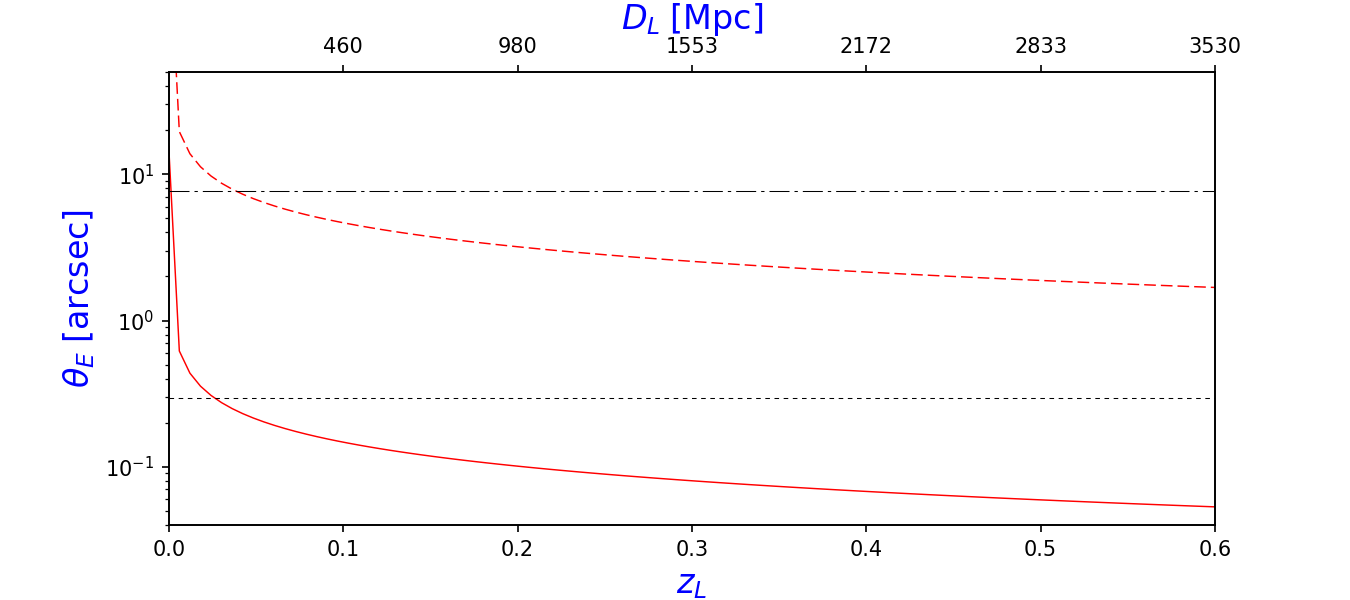
\includegraphics[scale=0.8]{5_HALOS/radio_einstein.png}
      \caption{\small Variación del radio de Einstein con la distancia observador-lente (Ecuación \ref{eq:radio_einstein_magnitud}) suponiendo un objeto lente puntual de masa \masassolares{10^9}(curva roja continua) y masa \masassolares{10^{12}}(curva roja discontinua). La lineas horizontales representan los limites de resolución de los catálogos \hatlas\ (\maths{{\sigma}_{h}^{p}\sim7.63\;\mathrm{arcsec}}) y \gama\  (\maths{{\sigma}_{g}^{p}\sim0.297\;\mathrm{arcsec})}. El intervalo \maths{z_L} cubre el rango de valores que toma el \rt\ para la gran mayoría de los objetos del catálogo \gama\ (ver Figura \ref{fig:histograma_z_gama}). La escala que aparece sobre la parte inferior de la figura es el \rt\ equivalente a la distancia que aparece en la escala superior de la figura según el modelo Lambda-CDM \footnotemark. Obsérvese que la Ecuación \ref{eq:radio_einstein_magnitud} relaciona \maths{\theta_E} con \maths{D_L}, no con \maths{z_L} que es lo que se mide directamente a partir de la observación del objeto.}
  \label{fig:radio_einstein}
  \end{center}
\end{figure}
\footnotetext{Para realizar este cálculo se ha utilizando el paquete \texttt{astropy.cosmology} y el modelo Lambda-CDM (Lambda Cold Dark Matter) con valor de la constante de Hubble 70 \maths{\mathrm{km\;{s}^{-1}\;{Mpc}^{-1} }} y densidad de la materia no relativista en unidades de la densidad crítica \maths{\Omega_{0}}=0.3.}

Nosotros no esperamos encontrar anillos de Einstein, pero los emparejados que estamos buscando forman lentes gravitatorias fuertes y sabemos que separación angular entre nuestros candidatos a lente gravitatoria debe ser de ese orden de magnitud. Teniendo en cuenta el radio efectivo de una galaxia elíptica de gran tamaño, su masa y un desplazamiento al rojo \maths{z\sim0.1}, cabria esperar una separación angular de \maths{\sim17\:\mathrm{arcsec}}. Dado que se trata de un caso extremo para una galaxia especialmente grande y especialmente próxima el resto de candidatos deben mostrar separaciones angulares inferiores.

La idea del método que proponemos es encontrar lentes gravitatorias en un subconjunto de emparejados que surgen al aplicar el método de \cross\ de catálogos de galaxias descrito en la sección anterior al considerar los catálogos \hatlas y \gama. Se trata de observaciones que dada su proximidad angular podrían pertenecer al mismo objeto, pero que sin embargo tienen \rts\ diferentes (esto es equivalente a decir que se cumplen las condiciones \maths{B^{p}_{12}>1} y \maths{B_{12}<1}).
Como hemos visto en la Sección~\ref{sec:4_cross_identificacion}, dada la resolución angular de los catálogos utilizados, el factor de Bayes posicional considerado toma el valor 1 cuando la separación angular de dos observaciones se encuentra en  \maths{\sim49.64\;\mathrm{arcsec}}. Esta distancia angular es varias veces mayor que la distancia de angular máxima que estimamos para la lente gravitatoria. Esto resulta beneficioso por una parte porque de esta manera probablemente la mayor parte de las lentes gravitatorias cuando intervienen dos objetos pertenezcan a este conjunto, pero también es un problema porque si la distancia de emparejamiento es muy grande, se incrementará también el número de contrapartidas formadas por observaciones entre objetos que no guardan ningún tipo de relación entre sí. Lo ideal sería que la distancia para la cuál \maths{B_{12}^{p}=1} se encontrase en \maths{\sim17\:\mathrm{arcsec}}.

A modo de resumen, el procedimiento que se va a seguir en este trabajo para identificar lentes gravitatorias será el siguiente: 

\vspace{-3mm}

\begin{itemize}
    
    \item Seleccionaremos todas aquellas observaciones de los catálogos \hatlas\ y \gama\ de los cuales disponemos una medida razonable de su \rt \footnote{Por medida razonable del \rt\ entendemos, una medida del \rt\ proporcionada por los catálogos o una estimación válida obtenida mediante el método descrito en la Sección~\ref{sec:3_redshift_hatlas}. Obsérvese este método solo sirve para galaxias lejanas en formación. Estos objetos son abundantes a \rts\ altos, pero no son los únicos. El método propuesto para la identificación de lentes gravitatorias no depende de si las fuentes son ETGs o no.}.
    
    \item Partiendo de la selección anterior, se realizará una búsqueda exhaustiva de todos las las observaciones del catálogo \hatlas\ DR1 que se encuentran a una distancia inferior a los \maths{\sim49.64\;\mathrm{arcsec}} de otro de \gama. En realidad, en este trabajo se ha escogido una distancia de emparejamiento de \maths{54\;\mathrm{arcsec}} y después se ha utilizado la condición de \maths{B^{p}_{12}<1}, pero esto es equivalente a elegir una distancia de emparejamiento de máxima de \maths{\sim49,64\;\mathrm{arcsec}} desde el principio.
    
    \item A cada emparejado, le asignaremos tres factores de Bayes: \maths{B^{p}_{12}}, \maths{B^{z}_{12}} y \maths{B_{12}}. Seleccionaremos aquellos que cumplen las condiciones de \maths{B^{p}_{12}>1} y \maths{B_{12}<1}.
    
    \item Por último seleccionaremos aquellos emparejados en los que \maths{z_{h}\!>\!1} (para poder considerar la observación perteneciente \hatlas\ un objeto con alto \rt ) y \maths{z_{h}>z_{g}} (ya que los objetos lente los buscamos en \gama\ y las fuentes en \hatlas ). La muestra resultante será nuestra selección de candidatos a sistemas lente gravitatoria en la que participa una fuente con un alto \rt.
    
\end{itemize}